\documentclass[11pt,a4paper]{report}
\usepackage{mathpazo}
\usepackage{graphicx,url}
\usepackage[usenames,dvipsnames]{color}
\usepackage[colorlinks=true,linkcolor=Blue,urlcolor=Blue,citecolor=Blue]{hyperref}
\usepackage{../../vpl}
\graphicspath{{../../images/}}
\usepackage[francais]{babel}% To be able to display accents and french stuff
\usepackage[T1]{fontenc} 
\usepackage[utf8]{inputenc}
\usepackage{lmodern}

\usepackage[tikz]{bclogo}
\usepackage{wrapfig}
\usepackage{listings} % Use for code listing: \begin{lstlisting}[frame=lines, caption={...}, label=...] ... code... \end{lstlisting} We can use \begin{minipage}{\linewidth} ... \end{minipage} to avoid page break

\usepackage{subfigure} %Allows the use of subfigure and subtable. Use like that: \subfigure[<list_entry>][<subcaption>]{<figure>} or \subtable[<list_entry>][<subcaption>]{<figure>}. You can't put other ']' character in the [..][..] parts. You can surround them with {} => not like [blabla $sqrt[3]{1}$ blabla] but like [blabla {$sqrt[3]{1}$} blabla]

\usepackage{cleveref} %Cross referencing and simplify referencing. Use \cref{..} or \Cref{..} in beginning of sentances. For a range of reference, use \crefrange{..}. To reference a page, use \cpageref{..}. Package has to be declared last!

%\includeonly{}

\newcommand{\crefrangeconjunction}{ à } % Redesign names to match with french

\renewcommand{\tablename}{Tableau}
\crefname{table}{le tableau}{les tableaux}
\Crefname{table}{Le tableau}{Les tableaux}

\renewcommand{\figurename}{Figure}
\crefname{figure}{la figure}{les figures}
\Crefname{figure}{La figure}{Les figures}

\crefname{equation}{l'équation}{les équations}
\Crefname{equation}{L'équation}{Les équations}

\crefname{chapter}{le chapitre}{les chapitres}
\Crefname{chapter}{Le chapitre}{Les chapitres}

%\crefname{lstlisting}{listing}{listings}
%\Crefname{lstlisting}{Listing}{Listings}

%\pagenumbering{Roman} \setcounter{page}{0} 
%\thispagestyle{empty}
%%\includepdf{Images/Premiere_page}
%
%\tableofcontents
%
%\newpage
%\pagenumbering{arabic} \setcounter{page}{1}

\begin{document}
\pagenumbering{Roman} \setcounter{page}{0} 
\thispagestyle{empty}

\begin{center}
\begin{LARGE}
\begin{bfseries}
Premiers pas en robotique

avec le robot

Thymio-II

et l'environnement
\vspace{0.5cm}
Aseba/VPL
\end{bfseries}
\end{LARGE}

\bigskip\bigskip

\begin{Large}
Version 1.0 pour \href{https://aseba.wikidot.com/en:downloadinstall}{Aseba 1.3.1}
\end{Large}

\bigskip\bigskip

\begin{LARGE}
\href{http://www.weizmann.ac.il/sci-tea/benari/}{Moti Ben-Ari} et autres contributeurs\\
\end{LARGE}
\bigskip
\begin{Large}
voir \texttt{authors.txt} pour plus de détails
\end{Large}

\vspace{1cm}

\begin{Large}
Traduis de l'anglais au français par Christophe Barraud
\end{Large}

\bigskip


\end{center}

\vfill

\begin{center}
\copyright{}\  2013 par \href{http://www.weizmann.ac.il/sci-tea/benari/}{Moti Ben-Ari} et autres contributeurs. Traduis de l'anglais au français par Christophe Barraud
\end{center}

%This work is licensed under the Creative Commons
%Attribution-ShareAlike 3.0 Unported License. To view a copy
%of this license, visit
%\url{http://creativecommons.org/licenses/by-sa/3.0/}
%or send a letter to Creative Commons, 444 Castro Street, Suite 900,
%Mountain View, California, 94041, USA.

\begin{center}

\includegraphics[width=.2\textwidth]{../images/by-sa}
\end{center}

\tableofcontents
\thispagestyle{empty}

% !TeX root = vpl.tex

\chapter*{Preface}

\sect{What is a robot?}

You are riding your bicycle and suddenly you see that the street starts
to go uphill. You pedal faster to supply more power to the wheels so
that the bicycle won't slow down. When you reach the top of the hill and
start to go downhill, you squeeze the brake lever. This causes a rubber
pad to be pressed against the wheel and the bicycle slows down.
When you ride a bicycle, your eyes are \textit{sensors} that sense what is
going on in the world. When these sensors---your eyes---detect an
\textit{event} such as a curve in the street, you perform an
\textit{action}, such as moving the handlebar left or right.

In a car, there are sensors that \textit{measure} what is going on in the
world. The speedometer measures how fast the car is going; if you see it
measuring a speed higher than the limit, you might tell the driver that
he is going too fast. In response, he can perform an action, such as
stepping on the brake pedal to slow the car down. The fuel meter
measures how much fuel remains in the car; if you see that it is too
low, you can tell the driver to find a gas station. In response, she can
perform an action: raise the turn-signal lever to indicate a right turn
and turn the steering wheel in order to drive into the station.

The rider of the bicycle and the driver of the car receive data from
the sensors, decide what actions to take and cause the actions to be
performed. A \textit{robot} is a system where this process---receive data,
decide upon an action, perform the action---is carried out by a
computerized system, usually without the participation of a human.

\sect{The Thymio-II robot and the Aseba VPL environment}

The Thymio II is a small robot intended for educational purposes
(\cref{fig.front}). The robot includes sensors that can measure
light, sound and distance, and can detect when buttons are touched and
when the robot's body is tapped. The most important action that it can
perform is to move using two wheels, each powered by its own motor.
Other actions include generating sound and turning lights on and off.

In the rest of this document, the Thymio~II robot will be called simply Thymio.
It will always refer to the version II of the robot.

Aseba is a programming environment for small mobile robots such as the Thymio.
VPL is a component of Aseba for \textit{visual programming} that was designed to program Thymio in an easy way through event and action blocks.
This tutorial assumes that you have Aseba installed on your computer; if it is not the case, go to \url{https://aseba.wikidot.com/en:downloadinstall}, select your operating system, download and install.



\pagenumbering{arabic} \setcounter{page}{1}
\part{Tutorial}

\chap{Your First Robotics Project}\label{ch.intro}

\sect{Getting to know your Thymio}

\Cref{fig.front} shows the front and top of Thymio. On the top you
can see the center circular button (\textcolor{blue}{A}) and four
directional buttons (\textcolor{blue}{B}). Behind the buttons, the green
light (\textcolor{blue}{C}) shows how much charge remains in the
battery. At the back are the top lights (\textcolor{blue}{D}), which
have been set to red in this picture. There are similar lights on the
bottom (see \cref{fig.bottom}). The small black rectangles
(\textcolor{blue}{E}) are sensors which you will learn about in
\cref{ch.pet}.

\begin{figure}[h]
\begin{center}
\gr{front}{.8}
\caption{The top and front of the Thymio robot}\label{fig.front}
\end{center}
\end{figure}

\sect{Connect the robot and run VPL}

Connect your Thymio robot to your computer with a USB cable; the robot
will play a sequence of tones. If the robot is turned off, turn it on by
touching the center button for a few seconds until you hear the tones.
Run VPL by double-clicking on the icon \blksm{thymiovpl} on your
computer.

\importantbox[Small images]{When a small image appears
in the text, a larger image is displayed in the margin.}

VPL may connect automatically to your robot. If not, the window shown in
\cref{fig.connect} will be displayed. Check the box next to \bu{Serial},
click on \bu{Thymio Robot} below it, select a language, and then click
\bu{Connect}. Depending on the configuration of your computer and
operating system, there may be several entries in this table and the
data following \bu{Thymio Robot} may be different from what is shown in
the Figure.

\trickbox{It is also possible to access VPL from Aseba Studio, the
text-based programming environment through the VPL plugin found in the
\textit{Tool} area at the bottom left of the screen.}

\begin{figure}
\begin{center}
\gr{connect}{.4}
\caption{Connect to Thymio through serial port (USB)}\label{fig.connect}
\end{center}
\end{figure}

\newpage

\sect{The VPL user interface}

The user interface of VPL is shown below.
There are six areas in the interface:
\begin{enumerate}[noitemsep,nosep]
\item A toolbar with buttons for opening, saving, running a program, etc.
\item A program area where programs for controlling the robot are constructed.
\item A message area which displays error messages if the program is not
well-formed.
\item A column with event blocks for constructing your program.
\item A column with action blocks for constructing your program.
\item The translation of the program into AESL, the textual language of Aseba.
\end{enumerate}

\plainfloat
\begin{figure}[h]
\gr{gui}{1}
\caption{The VPL window}\label{fig.vplgui}
\end{figure}
\framedfloat

\bigskip

\informationbox{To go further}{ When you construct a program using VPL, the
translation of the program into the textual programming language AESL
appears in the right part of the window. It is the AESL program that is
actually run by the robot. If you are curious and wish to understand
AESL, you can read the \cref{ch.next} which explains these translations.
Then, go to
\href{https://www.thymio.org/en:asebausermanual}{https://www.thymio.org/en:asebausermanual}
for learning and reference materials on AESL and its Studio
environment.}

\newpage

\sect{Write a program}

When you start VPL, a blank program area is displayed.

If, after having built a piece of program, you wish to clear the content
of the program area, click \blksm{new} (\bu{New}).

A program in VPL consists of \emph{event-actions pairs}, each
constructed from an event block and one or more action blocks. For
example, the pair: \blkc{e-a-pair} causes the top light of the robot to
display red when the front button is touched.

\importantbox[Meaning of an event-actions pair]{\centering When the event
occurs, the associated actions are run.}

The program area will initially contain an empty frame for an
event-actions pair: \blkc{empty-frame} To bring a block to the program
area from the colums (areas 4 and 5 of \cref{fig.vplgui}), press and
hold the left mouse button and drag the block to a dashed square. When the
block is over the square, release the mouse button, dropping the event block
into its place.

\importantbox{The technique just described is call
\emph{drag-and-drop} and is widely used in the user interface of
programs.}

Start by bringing the button event block \blksm{event-buttons} into the
left side of the empty frame. You will get a message inviting you to add
an action block. Drag the top color action block
\blksm{action-colors-up} and drop it into into the right side of the frame. You have
constructed an event-actions pair!

Next, we have to modify the event and the action to do what we want. For
the event, click on the front button (the top triangle); it will turn
red: \blkc{forward} This specifies that an event will occur when the
\textit{front button} of Thymio is touched.

The color action block contains three \emph{sliders}---colored bars with
a white square---one for each of the primary colors red, green, blue.
Drag a white square to the right and then back to the left, and you will
see that the background color of the block changes. All colors can be
made by mixing these three primary colors: red, green and blue. Move
the red slider until the square is at the far right, and move the green
and blue sliders until they are at the far left. The color will be all
red with no blue nor green: \blkc{red}

\sect{Save the program}

Before running the program, save it on your computer. Click on the
button \blksm{save} (\bu{Save}) in the toolbar. You will be asked to
give the program a name; choose a name that will help you remember what
the program does, perhaps, \bu{display-red}. Choose the location where
you want to save your program and click on \bu{Save}.


\importantbox[Save frequently]{When you modify a program, click
\bu{Save} frequently so that you don't lose your work if something
happens to the computer.}


\sect{Run the program}

To run the program, click on \blksm{run} (\bu{Run}) in the toolbar.
Touch the front button on the robot; the light on top of the robot
should change to red.

\informationbox{Congratulations!}{You have created and run your
first program. Its behavior is:\\ \textbf{When you touch the forward
button of the Thymio, it becomes red.}}

If you need to stop the VPL program, click \blksm{stop} (\bu{Stop}) .
This is important when you run a program that causes the robot to move,
but the program does not have an event-actions pair to stop the motors.

\sect{Turn the robot off}

When you have finished working with the Thymio robot, you can turn it
off by touching and holding the center button for a few seconds until
you hear a sequence of tones. The battery in the robot will
continue charging as long as it is connected to a working computer. A
red light next to the USB cable connector means that the robot is
charging; it turns blue when the charging is completed (\cref{fig.back}).
You can disconnect the cable when you are not using the robot.

\trickbox{You can charge the robot faster by using a mobile phone
charger with a micro-USB connector.}

\begin{figure}
\begin{center}
\gr{back}{.6}
\caption{The back of the Thymio showing the USB cable and the
 charging light}\label{fig.back}
\end{center}
\end{figure}

Should the USB cable disconnect during programming, VPL will wait for
the connection to be made again. Check both ends of the cable, reconnect
and see if VPL is working. If you have a problem, you can always close
VPL, reconnect the robot and open VPL again.

%\newpage

\sect{Modify a program}

\begin{itemize}

\item To delete an event-actions pair, click \blkxsm{x} at the top-right
of the pair.

\item To add an event-actions pair, click \blkxsm{plus} available below
an existing pair.

\item To move an event-actions pair to another position in the program,
drag and drop it at the desired location.

\item To copy an event-actions pair to another position in the program,
press and hold the \bu{Ctrl} and then use the mouse to drag and drop the
pair at the desired location.\label{p.copy-pairs}\footnote{On Mac
OS, the \bu{Command} button is used instead of \bu{ctrl}.}

\end{itemize}

\informationbox{The blinking \bu{Run} button}{When you modify a program,
the \bu{Run} button blinks blue and green to remind you that you need to
click the button to load the modified program into the Thymio
robot.\label{p.blink}}

If you want to experiment with a modification but not lose an existing
program, you can create a copy of the existing program by clicking
\blksm{saveas} and giving a new file name.

\sect{Open an existing program}

Suppose that you have saved your program and turned off the robot and
the computer, but later you wish to continue to work on the program.
Connect the robot and run VPL as described previously. Click on
\blksm{open} (\bu{Open}) and select the program you want to open, for
example, \bu{display-red}. The event-actions pairs of the program will
be displayed in the program area, and you can continue working on it.

\newpage

\sect{The current event-actions pair}

When you click on an event-actions pair, it will be displayed with a
yellow background. This will also occur when you enter an event or
action block in an empty pair:

\begin{center}
\begin{tabular}{c@{\hspace{.1\textwidth}}c}
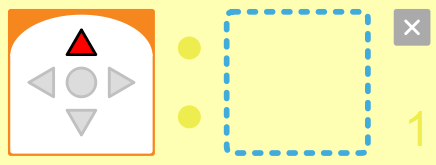
\includegraphics[width=.3\textwidth,keepaspectratio=true]{event-action-pair-yellow1}
&
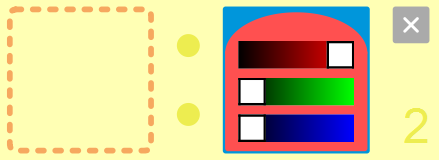
\includegraphics[width=.3\textwidth,keepaspectratio=true]{event-action-pair-yellow2}
\end{tabular}
\end{center}

The left gold-colored square is the space for the event; the right
blue-colored square is for the first (or only) action. The pair with the
yellow background is called the \emph{current} pair.

\informationbox{Quick entering of a block}{If you click on an event or action block, it will be
automatically placed in the program area in the current
event-actions pair.}

\bigskip

\bigskip

\informationbox{The VPL toolbar}{\cref{a.toolbar} contains a
description of all the buttons in the VPL toolbar. Look at it
occasionally until you have learned how to use them.}

\chap{Changer les couleurs}

\sect{Colorer Thymio}

\begin{bclogo}[couleur = pink!30, arrondi = 0.1, logo = \bccrayon, ombre = true]{Challenge!}Écrivez un programme en utilisant VPL qui affiche deux couleurs différentes sur le dessus de Thymio lorsque le bouton avant ou arrière est pressé et deux autres couleurs sous Thymio lorsque le bouton gauche ou droite est pressé.
\end{bclogo}

{\raggedleft \hfill Programme: \bu{colors.aesl}}

Nous avons besoin de quatre paires d'événement-action puisqu'il y a quatre conditions. Les quatre événements sont la pression des quatre boutons en forme de triangle de Thymio. Chacun de ces événements doit être associé avec une action de couleur. Vous verrez qu'il y a une différence entre l'icône \blk{action-colors-up-white} et l'icône \blk{action-colors-down-white}. La première des deux affiche une couleur sur le dessus de Thymio alors que la deuxième allume le dessous de Thymio. En effet, sur la deuxième icône, nous voyons les roues de Thymio!

Le programme est illustré sur \cref{fig.colors-a}.

Quelles couleurs seront affichées? Pour la première paire événement-action, le \textit{slider} de la couleur rouge a été glissé tout à droite alors que les autres sont restés à gauche, donc Thymio sera illuminé en rouge. La deuxième et troisième paire affichera respectivement du bleu et du vert. Quant à la dernière paire, elle affichera du jaune! Avec ces trois \textit{sliders}, il est donc possible de créer n'importe quelle couleur!  Vous pouvez voir que l'icône d'action couleur de Thymio se colorie en fonction de la position des \textit{sliders}, cela vous montre de quelle couleur sera Thymio!

Lancez le programme et vérifiez que les événements déclenchés par les boutons sont bien suivis des actions correspondantes.

\Cref{fig.front} montre Thymio illuminé en rouge sur le dessus et \cref{fig.bottom} montre Thymio illuminé en vert par le dessous.

\sect{Éteindre les lumières}

Modifions maintenant le programme pour que les lumières s'éteignent lorsque le bouton central est pressé. Nous allons avoir besoin de deux paires événement-action, une pour éteindre les lumières du dessus de Thymio et une autre pour les lumières du dessous. En faisant glisser tous les \textit{sliders} sur la gauche, comme sur \cref{fig.colors-b}, la lumière sera éteinte. Vous voyez que l'événement est le même, appuyer sur le bouton centrale, mais l'action associée est différente, éteindre les lumières du haut ou du bas.

\begin{figure}[h]
    \centering
    \subfigure[Changer les couleurs lorsqu'un bouton flèche est pressé]{ \label{fig.colors-a} 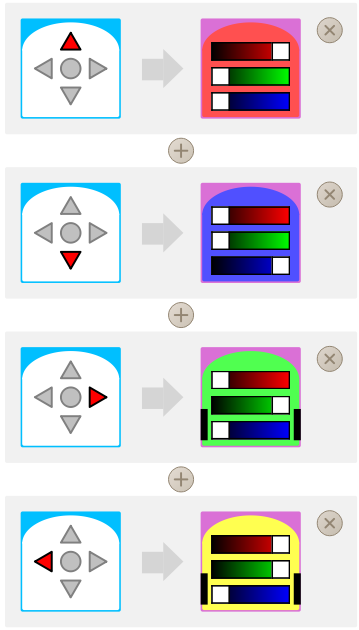
\includegraphics[width = 0.35\textwidth]{colors1}}
    \hspace{1cm}
    \subfigure[Éteindre Thymio lorsque le bouton centrale est pressé]{ \label{fig.colors-b} 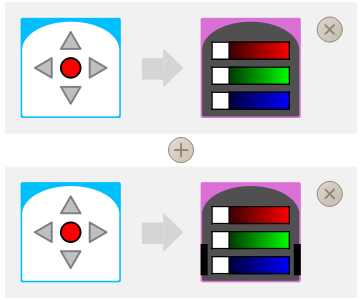
\includegraphics[width = 0.35\textwidth]{colors2}}
    \caption{Jouer avec les lumières de Thymio}
    \label{fig.colors}
\end{figure}

\begin{bclogo}[couleur = blue!30, arrondi = 0.1, logo = \bcinfo, ombre = true]{Trucs et astuces!}Lorsqu'un programme est lancé, toutes les paires d'événement-action sont actives.

Il est possible d'avoir plusieurs fois le même événement mais il \textbf{faut} que l'action correspondante soit différente! Si l'événement et l'action sont identiques, VPL vous indiquera qu'il y a une erreur.
\end{bclogo}





\chap{Thymio en mouvement}\label{Chap.Thymio.bouge}

\sect{En avant, en arrière}

Thymio a deux moteurs, un sur chaque roue. Ils peuvent tourner dans les deux sens, permettant à Thymio d'avancer, de reculer et de tourner. Commençons par un petit programme qui vous apprendra à contrôler les moteurs.

Le bloc d'action des moteurs représente Thymio entouré de deux \textit{sliders}: \blk{action-motors} 

Chaque \textit{slider} contrôle un moteur. En les faisant glisser vers l'avant, Thymio avancera, à l'inverse, en les faisant glisser vers l'arrière, Thymio reculera. Pour arrêter le moteur, il suffit de glisser les \textit{sliders} au centre des barres. Finalement, pour faire tourner Thymio, il suffit de faire avancer les moteurs avec des vitesse différentes!

\begin{bclogo}[couleur = pink!30, arrondi = 0.1, logo = \bccrayon, ombre = true]{Challenge!}Écrivez un programme en utilisant VPL qui fasse avancer Thymio lorsque le bouton avant est pressé et qui le fait reculer si vous appuyer sur le bouton arrière!
\end{bclogo}

{\raggedleft \hfill Programme \bu{moving.aesl}}

Nous allons avoir besoin de deux paires événement-action. Une pour faire avancer Thymio, l'autre pour le faire reculer, comme sur \cref{fig.nostop}. Faites glisser les blocs correspondants dans le canevas, réglez le bouton que vous souhaitez utiliser et ajustez les \textit{sliders} des moteurs pour faire avancer Thymio dans un cas et pour le faire reculer dans l'autre. Plus vous tirerez les \textit{sliders} vers l'avant ou l'arrière, plus les moteurs tourneront vite. Essayez d'abord avec une vitesse moyenne.

Démarrez maintenant le programme en cliquant sur \blksm{run} et touchez les boutons avant et arrière pour voir si Thymio avance et recule!

\begin{figure}
\begin{center}
\gr{no-stop-motors}{.4}
\caption{Thymio avance et recule}\label{fig.nostop}
\end{center}
\end{figure}

\sect{Arrête-toi!}

Avec ce programme, Thymio ne veut plus s'arrêter. Nous allons arranger cela en ajoutant une paire événement-action dans le programme. Avec ces deux blocs, Thymio s'arrêtera lorsqu'on presse son bouton centrale: \blk{stop-motors}. Lorsque vous ajoutez un bloc moteur dans le programme, il vient directement avec les \textit{sliders} réglés pour que les moteurs s'arrêtent.

\begin{bclogo}[couleur = blue!30, arrondi = 0.1, logo = \bcinfo, ombre = true]{Trucs et astuces!}Thymio s'arrêtera si vous cliquez sur \blksm{stop}
\end{bclogo}

\sect{Ne tombe pas de la table}

Si Thymio se trouve sur le sol, au pire, il rentrera dans un mur ou se débranchera tout seul de votre ordinateur, mais s'il est sur une table, il risque de tomber! Nous allons créer un petit programme qui lui permettra de s'arrêter s'il arrive au bord de la table.

\begin{bclogo}[couleur = green!30, arrondi = 0.1, logo = \bctakecare, ombre = true]{Attention!}Si Thymio roule sur une table, tenez vous toujours prêt à le rattraper s'il arrive près du bord de la table!
\end{bclogo}

Tournez Thymio sur son dos. Vous verrez deux petits rectangles noirs qui contiennent des éléments optiques, comme nous le voyons sur le haut de \cref{fig.bottom}. Ce sont les \textbf{détecteurs de sol}! Ils envoyent une impulsion de lumière et mesure la quantité de lumière qui leur est réféchie. Si Thymio est posé sur une table de couleur claire, beaucoup de lumière sera réfléchie, alors que s'il est sur le dos, comme sur \cref{fig.bottom}, ou qu'il dépasse le bord de la table, peu de lumière sera réfléchie. Nous allons donc utiliser ces capteurs pour dire à Thymio de s'arrêter lorsqu'il arrive au bord de la table.

\begin{bclogo}[couleur = blue!30, arrondi = 0.1, logo = \bcinfo, ombre = true]{Trucs et astuces!}Évitez les tables en verre transparent, elle ne réfléchiront pas la lumière et Thymio croira qu'il n'est pas sur une table!
\end{bclogo}

Tirez le bloc \textbf{détecteur de sol} sur le canevas pour commencer: \blk{event-ground}. Les deux petits carrés gris représentent les détecteurs de sol. En cliquant sur ces carré, ils passent de gris à rouge, à blanc puis à nouveau à gris, etc. Ces couleurs signifient:

\begin{description}
	\item[Gris] \hfill \\
		Le détecteur n'est pas utilisé
	\item[Rouge] \hfill \\
		L'action associée est déclenchée s'il y a beaucoup de lumière réfléchie
	\item[Blanc] \hfill \\
		L'action associée est déclenchée s'il y a peu de lumière réfléchie
\end{description}

Pour faire en sorte que Thymio s'arrête au bord de la table, il faut ajouter au programme précédent une paire événement-action qui lui dit qu'il doit s'arrêter si ses détecteurs de sol ne voient que peu de lumière réfléchie, comme suit: \blk{dont-fall}.

\begin{figure}
\begin{center}
\gr{bottom}{0.6}
\caption{Le dessous de Thymio avec ses détecteurs de sol}\label{fig.bottom}
\end{center}
\end{figure}

Placez Thymio près d'un bord d'une table de façon à ce qu'il fasse face au bord et appuyez sur le bouton avant. Il devrait avancer jusqu'au bord et s'y arrêter. 

\begin{bclogo}[couleur = blue!30, arrondi = 0.1, logo = \bcinfo, ombre = true]{Trucs et astuces!}Si vous voulez arrêter le Thymio un peu avant le bord de la table, vous pouvez placer une feuille noir, ou du scotch noir, là où vous souhaitez qu'il s'arrête! 
\end{bclogo}

\begin{bclogo}[couleur = pink!30, arrondi = 0.1, logo = \bccrayon, ombre = true]{Challenge!}Jouez avec le contrôle des moteurs de Thymio. À sa vitesse maximale, est-il toujours capable de s'arrêter avant le bord de la table?
\end{bclogo}
\chap{Un robot de compagnie}\label{ch.pet}

Un \textit{robot autonome} adopte un comportement spécifique en fonction de la situation dans laquelle il se trouve. Il réussi à réagir grâce au \textit{feedback}, littéralement de l'information en retour. Il faut donc que le robot puisse "voir" le monde qui l'entoure pour pouvoir y régir.

\sect{Thymio vous obéit}

Pour commencer, nous allons apprivoiser Thymio pour qu'il vous obéisse. 

\begin{bclogo}[couleur = pink!30, arrondi = 0.1, logo = \bccrayon, ombre = true]{Challenge!}Écrivez un programme en utilisant VPL qui fait avancer Thymio lorsque vous mettez votre main devant lui!
\end{bclogo}

Il y a cinq capteurs de distance à l'avant de Thymio et deux à l'arrière. Ce sont les même que ceux qui se trouve sous Thymio et que nous avons utilisé pour détecter une table! Avancez votre main en direction des capteurs à l'avant de Thymio, vous verrez une lumière rouge apparaître à côté du capteur qui vous aura détecté, comme sur \cref{fig.detect}.

\begin{figure}
\begin{center}
\gr{detect}{.6}
\caption{L'avant de Thymio. Deux doigts sont détectés par les capteurs avant.}\label{fig.detect}
\end{center}
\end{figure}

Le bloc \blk{event-prox} sert à utiliser les capteurs avants et arrières de Thymio. Les cases sont utilisées comme pour les détecteurs situés sous Thymio. En cliquant dessus, ils passent de gris à blanc, à rouge et à nouveau à gris. Vous trouverez les significations des couleurs en dessous:

\begin{description}
	\item[Gris] \hfill \\
		Le détecteur n'est pas utilisé
	\item[Rouge] \hfill \\
		L'événement associé est déclenché si un objet se trouve proche de Thymio
	\item[Blanc] \hfill \\
		L'événement associé est déclenché si aucun objet ne se trouve proche de Thymio
\end{description}

Pour faire avancer Thymio si votre main est proche de lui et le faire s'arrêter si elle est loin, il nous faudra deux paires événement-action, comme sur \cref{fig.follow-hand}. La première dit à Thymio de s'arrêter s'il ne détecte rien devant lui grâce au bloc capteur où le carré central est blanc et au bloc moteur dont les \textit{sliders} sont au centre des barres. La deuxième paire dit qu'il doit avancer s'il voit quelque chose devant lui grâce au bloc capteur où le carré central est rouge et au bloc moteur avec les \textit{sliders glissés vers le haut}.

\begin{figure}[h]
\begin{center}
\gr{likes-forward}{.4}
\caption{Thymio avance vers votre main}\label{fig.follow-hand}
\end{center}
\end{figure}

\sect{Faire tourner Thymio}

Thymio n'est pas comme une voiture, il n'a pas de volant, ni de roues directrices. Pour tourner, il doit simplement faire tourner une de ses roues plus vite que l'autre! On appelle cela la \textbf{direction différentielle}, ou \textbf{differential drive}. Cette façon de se diriger est utilisée par de nombreux véhicules, comme par exemple le bulldozer de \cref{fig.bull}.

\begin{figure}
\begin{center}
\gr{bulldozer}{0.25}
\caption{Un bulldozer qui utilise aussi  la \textbf{direction différentielle}}\label{fig.bull}
\end{center}
\end{figure}

Si la roue droite tourne plus vite que la roue gauche, alors Thymio tournera à gauche, tandis que si sa roue gauche tourne plus vite que sa roue droite, il tournera à droite. Plus la différence de vitesse est élevée, plus le virage sera serré. Et pour tourner sur lui-même, il lui suffit de faire tourner ses deux roues à la même vitesse mais dans des sens opposés!

En réglant le bloc vitesse avec les \textit{sliders} à des endroits différents, les roues de Thymio ne tourneront pas à la même vitesse, ce qui fera tourner le robot. Essayez de régler le bloc vitesse comme cela: \blk{turning}. Si vous chargez ensuite ce programme et appuyez sur le bouton central, Thymio devrait tourner sur lui-même. Vous pouvez toujours l'arrêter en appuyant sur \blksm{stop}.

\begin{bclogo}[couleur = blue!30, arrondi = 0.1, logo = \bcinfo, ombre = true]{Trucs et astuces!}Le bloc vitesse s'anime dès que vous régler les \textit{sliders} pour vous donner une idée du mouvement de Thymio!
\end{bclogo}

\sect{Thymio vous suit}

Un vrai animal de compagnie ne se contente pas de s'approcher ou de s'éloigner de vous, il vous suit un peu partout! 

\begin{bclogo}[couleur = pink!30, arrondi = 0.1, logo = \bccrayon, ombre = true]{Challenge!}Écrivez un programme en utilisant VPL qui fasse avancer Thymio lorsque vous mettez votre main devant lui et qui le fasse tourner si vous tournez autour de lui!
\end{bclogo}

{\raggedleft \hfill Programme \bu{likes.aesl}}

Pour que Thymio puisse vous suivre plus fidèlement possible, il faudra ajouter deux paires événement-action au programme précédant. S'il vous détecte avec son capteur avant-droit, il doit tourner à droite et s'il vous détecte avec son capteur avant-gauche, il doit tourner à gauche.

Vous pouvez essayer différentes vitesses, le faire tourner sur lui-même ou non, afin de trouver le meilleur compromis! 

Une façon de faire est illustrée sur \cref{fig.likes}.

\begin{figure}
\begin{center}
\gr{likes-turns}{0.4}
\caption{Thymio s'oriente face à vous}\label{fig.likes}
\end{center}
\end{figure}

\sect{Thymio vous fuit}

Parfois, même le plus fidèle animal de compagnie n'a pas envie de vous suivre. 

\begin{bclogo}[couleur = pink!30, arrondi = 0.1, logo = \bccrayon, ombre = true]{Challenge!}Écrivez un programme en utilisant VPL qui fasse reculer Thymio lorsque vous mettez votre main devant lui et qui le fait vous éviter si vous lui tournez autour!
\end{bclogo}

{\raggedleft \hfill Programme \bu{does-not-like.aesl}}

Pour réussir à donner ce  comportement à Thymio, il suffit simplement de régler les moteurs sur la marche arrière s'il vous détecte avec son capteur avant et d'échanger les événements des paires d'événement-action restantes du programme précédant, comme sur \cref{fig.recule-evite}.

\begin{figure}[h]
    \centering
    \subfigure[S'il vous détecte devant lui, il recule]{ \label{fig.recule} 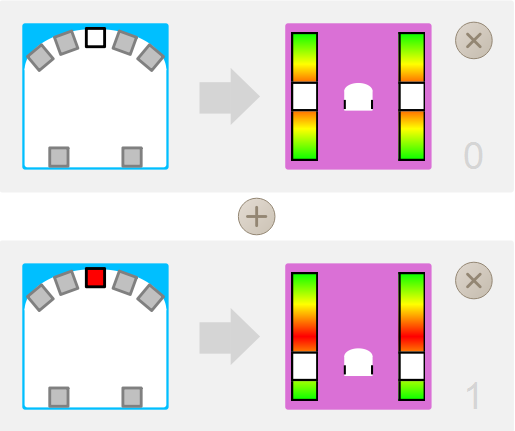
\includegraphics[width = 0.35\textwidth]{Thymio-flees}}
    \hspace{1cm}
    \subfigure[S'il vous détecte sur les côtés, il vous évite]{ \label{fig.evite} 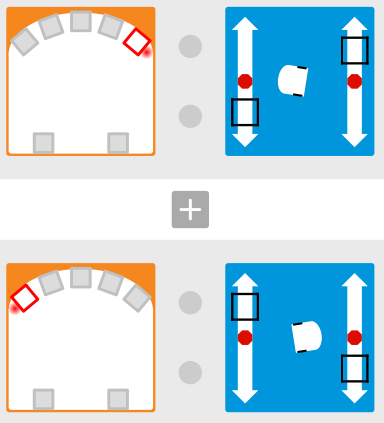
\includegraphics[width = 0.35\textwidth]{hates}}
    \caption{Thymio vous évite et vous fuit}
    \label{fig.recule-evite}
\end{figure}

\begin{bclogo}[couleur = pink!30, arrondi = 0.1, logo = \bccrayon, ombre = true]{Challenge!}Jouez avec les différents capteurs avant de Thymio. Vous pouvez utiliser les capteurs jusque là inutilisés pour améliorer le comportement de Thymio!
\end{bclogo}

\sect{Régler les \textit{sliders} plus précisément (avancé)}

Ce n'est pas très facile de régler les \textit{sliders} précisément pour, par exemple, faire avancer Thymio tout droit. Si vous regardez dans la fenêtre principale d'Aseba, vous verrez que le code qui sera transmis à Thymio s'écrit tout seul dès que vous remplissez les paires événement-action dans VPL. En comprenant un peu ce code et en le modifiant directement, il est possible d'ajuster plus précisément les vitesse des roues!

Le \cref{Follower_code} avec la figure d'à côté vous montre un exemple!

\begin{wrapfigure}{r}{0.24\textwidth}
  \begin{center}
    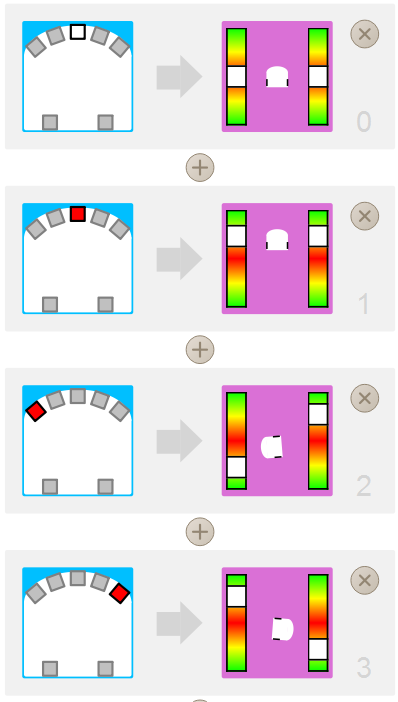
\includegraphics[width=0.24\textwidth]{follow4}
  \end{center}
\end{wrapfigure}

\begin{small}
\begin{lstlisting}[frame=single, caption={Thymio vous suit}, label=Follower_code, linewidth=9cm] 

onevent prox
	if prox.horizontal[2] < 400 then
		motor.left.target = 0
		motor.right.target = 0
	end
	if prox.horizontal[2] > 500 then
		motor.left.target = 300
		motor.right.target = 300
	end
	if prox.horizontal[0] > 500 then
		motor.left.target = -350
		motor.right.target = 350
	end
	if prox.horizontal[4] > 500 then
		motor.left.target = 350
		motor.right.target = -350
	end

\end{lstlisting}
	\end{small}

La ligne \p{onevent prox} signifie que le code qui suit sera lancé lorsque l'événement lié aux capteurs de proximité se produit. Cet événement est simplement une lecture de tous les capteurs qui a lieu dix fois par seconde!

Lorsque l'événement se produit, Thymio teste la valeur des capteur avec la condition: \p{if \ldots  then \ldots  end}. Il commence par tester le capteur numéro 2 comme nous le voyons avec la phrase \p{prox.horizontal[2]}. Si cette valeur est inférieure à 400, alors (\p{then}), Thymio règle la vitesse des moteurs gauche et droite à 0 avec les phrases: \p{motor.left.target = 0} et \p{motor.right.target = 0}.

Chaque bloc \p{if \ldots  then \ldots  end} teste un capteur spécifique et effectue ou non l'action associée. C'est exactement comme sur la figure à droite du \cref{Follower_code}.

\begin{enumerate}
	\item Thymio teste si rien ne se trouve devant lui, si c'est le cas, il s'arrête
	\item Thymio teste si quelque chose se trouve devant lui, si c'est le cas, il avance
	\item Thymio teste si quelque chose se trouve à sa gauche, si c'est le cas, il tourne à gauche
	\item Thymio teste si quelque chose se trouve à sa droite, si c'est le cas, il tourne à droite
\end{enumerate}

Nous voyons donc que chaque paire événement-action correspond à un bloc \p{if \ldots  then \ldots  end}!

Finalement, une fois que Thymio a testé tous ces capteurs, il attend le prochain événement \p{prox} et recommence ses tests, etc\ldots

Si vous voulez, vous pouvez essayer de modifier les nombres après les symboles $<$ ou $>$, ou ceux après les signes $=$. Chacun d'entre eux ont leur utilité et leurs limites, essayez de les comprendre!

Vous ne pourrez pas modifier le code écrit si VPL est ouvert. Sauvegardez votre travail sur VPL et quitter cette fenêtre pour commencer à jouer avec la programmation écrite!
\chap{Thymio est sur une piste}\label{ch.line}

Une promenade en montagne  peut sembler être une activité très simple. Il suffit d'enfiler une paire de chaussures de marche et de suivre le chemin. Pour un robot, suivre un chemin peut être très utile! Mais pour suivre un chemin, il faut encore le voir\ldots

\begin{bclogo}[couleur = pink!30, arrondi = 0.1, logo = \bccrayon, ombre = true]{Challenge!}Écrivez un programme en utilisant VPL qui permet à Thymio de suivre une ligne noire sur une table blanche!
\end{bclogo}

{\raggedleft \hfill Programme \bu{follow-line.aesl}}

Suivre une ligne sur le sol est un bon exemple du genre de difficultés rencontrées en robotique. La ligne peut-être mal dessinée, de la poussière ou de la saleté peuvent la recouvrir, le robot peut rencontrer des obstacles... Il faut donc créer, ce que nous appelons,  un contrôleur. Il aura pour tâche de dicter la vitesse du robot, sa direction, etc...

\sect{Quel genre de ligne}

Pour suivre une ligne, nous allons utiliser les détecteurs de sol que nous avons déjà utilisés dans \cref{Chap.Thymio.bouge}. Rappelons qu'il s'agit des mêmes capteurs que ceux qui se trouvent à l'avant et à l'arrière de Thymio. Ils envoient de la lumière infrarouge (invisible pour l'oeil humain) et analysent la quantité de lumière renvoyée.

Si vous poser Thymio sur une table blanche, ou du moins de couleur claire, beaucoup de lumière sera réfléchie, donc cet événement sera déclenché: \blk{lots-of-light}. Au contraire, si Thymio se trouve sur une surface foncée, noire par exemple, un peu de lumière sera réfléchie, c'est donc cet événement-ci qui sera déclenché: \blk{little-light}.

Pour détecter une ligne, Thymio doit donc suivre une trace sombre sur un environnement claire, ou l'inverse. Ce qui est important, c'est le contraste entre les deux environnements. Vous pouvez donc dessiner ou peindre une ligne noire sur une feuille blanche. Vous pouvez également utiliser un gros scotch noir que vous coller sur une table blanche ou un scotch blanc sur une table noir\ldots 

La ligne doit faire au minimum 5 centimètres de large pour que les deux capteurs sous Thymio puisse la détecter correctement. Vous pouvez voir un exemple sur \cref{fig.tape}.

\begin{figure}
\begin{center}
\gr{blacktape}{.5}
\caption{Thymio suit une ligne de scotch noir}\label{fig.tape}
\end{center}
\end{figure}


\begin{bclogo}[couleur = blue!30, arrondi = 0.1, logo = \bcinfo, ombre = true]{Truc et astuce!}Pour profiter pleinement des potentialités de Thymio, assurez-vous d'avoir un câble USB assez long, des rallonges peuvent être trouvées dans tous les magasins d'informatique.
\end{bclogo}

\sect{Thymio s'arrête, Thymio avance}

Le premier pas pour faire suivre une ligne à Thymio est de le faire avancer s'il est sur la ligne et de le faire s'arrêter s'il ne se trouve pas sur cette dernière. Comme expliqué précédemment, si Thymio se trouve sur une surface blanche, donc à côté de la ligne, beaucoup de lumière sera réfléchie sur ses capteurs inférieurs. Il faut donc qu'il s'arrête puisqu'il n'est pas sur la ligne. Ensuite, si Thymio se trouve sur la ligne, peu de lumière sera réfléchie sur ses capteurs inférieurs. Il faut donc le faire avancer s'il ne détecte que peu de lumière. Nous avons donc deux paires événement-action qui sont illustrées sur \cref{fig.start-stop}.

\begin{figure}[h]
\begin{center}
\gr{line-forward}{.3}
\caption{Thymio s'arrête, Thymio avance}\label{fig.start-stop}
\end{center}
\end{figure}

\sect{Votre premier contrôleur}

Maintenant, il s'agit de créer un contrôleur qui va faire suivre la ligne à Thymio. Le programme que vous avez fait jusqu'à maintenant fera s'arrêter Thymio dès qu'un de ses deux capteurs inférieurs verra qu'il n'est plus sur la ligne. Pour le faire suivre la ligne plutôt que s'arrêter dès qu'un des capteurs la quitte, il faut que: 

\begin{itemize}
	\item si Thymio se trouve à moitié sur la ligne, un peu trop à droite, il tourne à gauche afin de se remettre sur la ligne, comme illustré sur \cref{fig.too-right}.
	\item  si Thymio se trouve à moitié sur la ligne, un peu trop à gauche, il tourne à droite afin de se remettre sur la ligne.
\end{itemize}

Comme nous avons deux conditions, il nous faut deux paires événement-action, comme illustré sur\cref{fig.follow-line}.

\begin{figure}[h]
    \centering
    \subfigure[Thymio à moitié sur la ligne, vue du dessus]{ \label{fig.too-right} 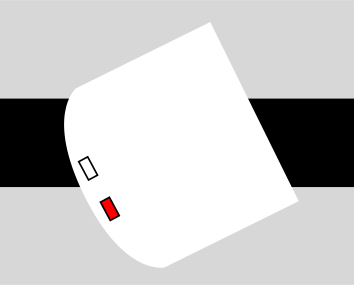
\includegraphics[width = 0.3\textwidth]{thymio_half_on_line}}
    \hspace{1cm}
    \subfigure[Trop à droite\ldots Trop à gauche]{ \label{fig.follow-line} 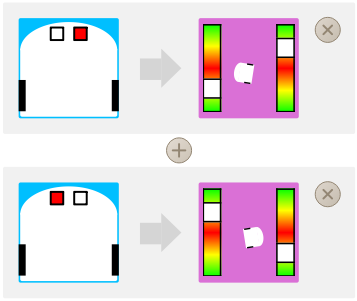
\includegraphics[width = 0.36\textwidth]{line-controller}}
    \caption{Un contrôleur pour suivre une ligne}
\end{figure}

\sect{Régler les paramètres}

Il est assez facile de comprendre que Thymio doit tourner à gauche s'il est trop à droite de la ligne et vis-versa. La vraie question est plutôt de combien doit-il tourner? Doit-il s'arrêter et tourner sur lui-même? Doit-il simplement corriger légèrement sa trajectoire? Ou au contraire le faire de manière plus sèche? C'est tout l'art de la création d'un contrôleur que de \textit{régler les paramètres} de ce contrôleur.

Mais quels sont ces \textit{paramètres}?

Ils varient totalement d'une application à une autre. Ils sont des entités que le créateur du contrôleur doit choisir afin d'obtenir le comportement désiré. Dans notre cas, il s'agit de la vitesse des roues dans les différents cas possibles. 

Thymio doit-il aller vite lorsqu'il est sur la ligne ou, au contraire, lentement? En allant vite, vous améliorerez son efficacité pour se déplacer d'un point à un autre mais vous risquez de le faire quitter la ligne avant qu'il ne s'en rende compte, un peu comme si vous allez trop vite en voiture dans un virage serré. Il faudra donc trouver un bon compromis pour le paramètre vitesse.

Une fois que Thymio remarque qu'il quitte la ligne, que doit-il faire? S'il s'arrête complètement et tourne sur lui-même, vous vous assurez qu'il ne quitte pas la ligne mais ses mouvements seront très saccadés. S'il corrige simplement sa trajectoire en diminuant la vitesse d'une roue, il se déplacera avec fluidité, mais il risque de quitter complètement la ligne\ldots 

Là aussi, il faudra trouver un bon compromis.

\begin{bclogo}[couleur = pink!30, arrondi = 0.1, logo = \bccrayon, ombre = true]{Challenge!}Thymio s'arrête complètement s'il ne détecte plus du tout la ligne. Modifiez le programme pour qu'il tourne lentement sur lui même s'il ne détecte plus du tout la ligne. Arrive-t-il à retrouver la ligne s'il la perd complètement? Essayer d'augmenter de plus en plus la vitesse des roues lorsqu'il est sur la ligne. Arrive-t-il à gérer un virage serré?
\end{bclogo}


\begin{bclogo}[couleur = pink!30, arrondi = 0.1, logo = \bccrayon, ombre = true]{Challenge!}Jouez avec la forme du parcours:

\begin{itemize}
\item Virages serrés
\item Virages doux
\item Zig-zag
\item Ligne plus large
\item Ligne plus étroite
\end{itemize}

Faites la course avec vos amis et votre famille. Qui arrive à faire le contrôleur le plus efficace? Y a-t-il un contrôleur parfait ou doit-il dépendre du parcours?
\end{bclogo}

\chap{Une petite pause}\label{ch.bells}

Faisons une pause avec les tâches compliquées et jouons un peu avec Thymio. Dans ce chapitre, nous vous montrerons que Thymio peut jouer de la musique, répondre à un son ou à un petite tape amicale!

\sect{Thymio mélomane}

Thymio possède un synthétiseur de sons qui lui permet de jouer des notes de musique! Vous pouvez le programmer simplement en utilisant le bloc action \blk{action-music}.

{\raggedleft \hfill Programme \bu{bells.aesl}}

Thymio peut jouer six notes différentes, chaque note doit être placée sur une barre de couleur représentant un ton. Il suffit de cliquer avec votre souris sur la barre de couleur de votre choix au niveau de la note que vous souhaitez modifier et voilà! Ensuite, vous pouvez choisir entre jouer une noire, un temps, et une blanche, deux temps, en cliquant sur la note que vous souhaitez modifier.

\Cref{fig.music} illustre deux chansons jouées par Thymio lorsque vous appuyez sur le bouton avant ou arrière.

\begin{figure}
\begin{center}
\gr{music}{.4}
\caption{Jouer une chanson}\label{fig.music}
\end{center}
\end{figure}

\begin{bclogo}[couleur = pink!30, arrondi = 0.1, logo = \bccrayon, ombre = true]{Challenge!}Écrivez un programme en utilisant VPL qui joue un thème connu!
\end{bclogo}

\sect{Thymio! Par ici!}

Thymio a un microphone, il peut donc réagir à un son! L'événement \blk{event-clap} se déclenche si Thymio entend un son fort, comme par exemple quelqu'un qui tape dans ses mains. 

En utilisant une paire événement-action avec l'événement \blk{event-clap} et le bloc d'action moteur, vous pouvez sans problème réaliser un programme qui fait avancer Thymio lorsque vous tapez dans vos mains.

\begin{bclogo}[couleur = blue!30, arrondi = 0.1, logo = \bcinfo, ombre = true]{Truc et astuce!}Si vous vous trouvez dans un environnement bruyant, il sera difficile pour Thymio de vous entendre.N'utilisez cette fonctionnalité que dans un environnement calme.
\end{bclogo}

\sect{C'est bien Thymio!}

Il est important de récompenser votre animal de compagnie quand il est gentil, c'est pareil avec Thymio! Il peut vous détecter si vous lui donner une petite tape sur la tête grâce à  l'événement: \blk{event-tap}. 

\begin{bclogo}[couleur = pink!30, arrondi = 0.1, logo = \bccrayon, ombre = true]{Challenge!}Écrivez un programme en utilisant VPL qui fasse s'approcher Thymio quand vous tapez dans vos mains et qui s'arrête et devienne rose si vous lui donner une petite tape sur la tête. Avec un seul microphone, Thymio n'arrivera pas à repérer l'origine du son, alignez-le donc dans votre direction.
\end{bclogo}

{\raggedleft \hfill Programme \bu{aux-pieds.aesl}}
\chap{Tout passe avec le temps}

Vous commencez à maîtriser Thymio, maintenant nous allons essayer de lui donner un comportement un peu plus complexe. En effet, Thymio va se vexer!

\begin{bclogo}[couleur = pink!30, arrondi = 0.1, logo = \bccrayon, ombre = true]{Challenge!}Écrivez un programme en utilisant VPL qui fait que Thymio soit content et devienne tout vert si vous touchez son bouton avant et qui se vexe en devenant tout rouge et en reculant durant quelques secondes si vous lui donnez une petite tape! Mais attention, au bout de quelques secondes, il doit vous avoir pardonné, s'être arrêté et être redevenu tout vert!
\end{bclogo}

{\raggedleft \hfill Programme \bu{vexe.aesl}}

Vous savez déjà comment faire faire devenir Thymio tout vert si vous appuyez sur son bouton avant. Vous savez aussi comment le faire devenir tout rouge et le faire reculer si vous lui donner une petite tape. Ce qui pose problème, c'est de le faire s'arrêter et redevenir tout vert \textit{après quelques secondes}.

Pour faire faire quelque chose à Thymio \textit{après quelques secondes}, il va falloir deux paires événement-action. Comme lorsque vous cuisiner et que vous ne voulez pas faire brûler votre gâteau, Thymio peut régler une alarme! 

Pour cela, il suffit d'utiliser le bloc alarme: \blk{action-timer}. Cette alarme est, en fait, un compte à rebours qui peut aller jusqu'à 4 secondes. Cette action peut-être déclenchée après n'importe quel type d'événement, par exemple après que Thymio ait ressenti une tape. Pour régler la durée du compte à rebours, vous pouvez cliquer dans le cadran de l'alarme et une petite animation vous montre combien de temps le compte à rebours va durer.

Si vous regardez les événements à gauche de la fenêtre du VPL, vous verrez un réveil qui sonne: \blk{event-timer}. Cet événement se déclanche dès qu'un compte à rebours arrive à zéro.

\begin{bclogo}[couleur = blue!30, arrondi = 0.1, logo = \bcinfo, ombre = true]{Truc et astuce!}En robotique, ce genre de compte à rebours s'appelle des \textit{timers}. Ils sont extrêmement utiles dans de nombreuses situations et vous verrez très vite à quel point!
\end{bclogo}

En déclenchant le compte à rebours lors d'un événement, comme une tape sur Thymio, et en associant une action, comme devenir vert, à l'événement de fin du compte à rebours, il est possible de créer un comportement qui se déclenche \textit{après quelques secondes}.

\Cref{fig.paire-timer} montre deux paires événement-action qui permettent d'allumer Thymio en vert quelques secondes après qu'on lui ait donné une petite tape.

\begin{figure}
\begin{center}
\gr{paire-timer}{.4}
\caption{Thymio s'allume en vert quelques secondes après avoir reçu une petite tape}\label{fig.paire-timer}
\end{center}
\end{figure}

Vous avez maintenant toute les clés en main pour réaliser le challenge de ce chapitre!

\chap{Modes: Pour ne pas toujours faire la même chose (avancé)}\label{ch.states}

Un programme VPL est composé d'une série de paires événement-action. Tous les événements sont vérifiés à tout moment et les actions appropriées sont effectuées. Ensuite, les événements sont vérifiés à nouveau, etc\ldots

Pour pouvoir programmer Thymio d'une façon un peu plus riche, il serait bien de pouvoir choisir quels événements sont à vérifier quand. Ainsi, il serait possible de créer des \textit{modes}. Thymio pourrait être en mode "recherche d'une ligne" ou en mode "suivi d'une ligne". Cela nous permettrait de programmer Thymio de deux façons différentes en une seule fois. Gardons cet exemple de la ligne. Si Thymio perd de vue la ligne, il pourrait se mettre à parcourir la région dans laquelle il se trouve en évitant d'éventuels obstacles jusqu'à ce qu'il la retrouve. Dès lors, il se remettrait en mode "suivi de ligne" et continuerait son chemin. Cela permettrait d'avoir une assurance pour qu'en cas de problème Thymio se débrouille tout seul!

Pour jouer avec les modes, commencez par cliquer sur le symbole avancé du VPL:   \blk{advanced}.


\sect{Toc, toc}

Dans les programmes que nous avons réalisé jusqu'ici, nous avons souvent \emph{démarré} Thymio en appuyant sur un de ces boutons et \emph{arrêté} Thymio en appuyant sur un autre. Mais regardez votre ordinateur. Normalement, il n'a qu'un seul bouton pour l'allumer ou l'éteindre. Il serait possible de faire deux actions avec un seul bouton si Thymio pouvait se souvenir que vous avez déjà appuyé ou non sur son bouton.

\begin{bclogo}[couleur = pink!30, arrondi = 0.1, logo = \bccrayon, ombre = true]{Challenge!}Écrivez un programme en utilisant VPL qui fasse que Thymio s'allume en rose si vous lui donnez une petite tape et qui fasse que Thymio s'éteigne si vous lui donnez une autre tape.
\end{bclogo}

{\raggedleft \hfill Programme \bu{tap-on-off.aesl}}

Nous allons décrire ce programme en utilisant un \textit{diagramme d'états}, comme sur \cref{fig.turn-on-off}.

\begin{figure}
\begin{center}
\gr{modes_diagramm}{0.3}
\caption{Diagramme d'état, \textit{allumé - éteint}}\label{fig.turn-on-off}
\end{center}
\end{figure}

Le diagramme de \cref{fig.turn-on-off} comprend deux modes, \textit{allumé} et \textit{éteint}. Chaque mode peut-être atteint en suivant une flèche. Depuis le mode \textit{allumé}, il est possible de se rendre au mode \textit{éteint} en passant par une flèche \textit{Toc}. À l'inverse, depuis le mode \textit{éteint}, il est possible de se rendre au mode \textit{allumé}, en suivant l'autre flèche \textit{Toc}. Les flèches symbolisent les paires événement-action. Une tape qui fait s'allumer Thymio le fait passer du mode \textit{éteint} au mode \textit{allumé}.

Ce diagramme peut-être \textit{traduit} en français comme:

\begin{itemize}
	\item \textbf{Si} Thymio est  \textit{allumé} et qu'il reçoit une \underline{tape}, \textbf{alors} Thymio devient \textit{éteint}.
	\item \textbf{Si} Thymio est  \textit{éteint} et qu'il reçoit une \underline{tape}, \textbf{alors} Thymio devient \textit{allumé}.
\end{itemize}

Ainsi, nous pouvons voir qu'un même événement, une tape, peut induire deux actions différentes, en fonction du mode dans lequel se trouve Thymio au moment de la tape.

Le programme complet est donné sur \cref{fig.state-changing} . Nous allons maintenant le détailler.

\begin{figure}[h]
    \centering
    \subfigure[Une tape pour allumer ou éteindre]{ \label{fig.state-changing-a} 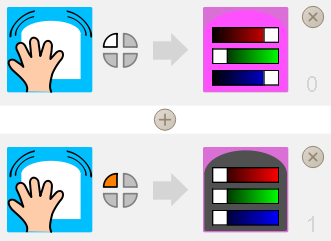
\includegraphics[width = 0.35\textwidth]{tap-on-off1}}
    \hspace{1cm}
    \subfigure[Une tape pour changer d'état]{ \label{fig.state-changing-b} 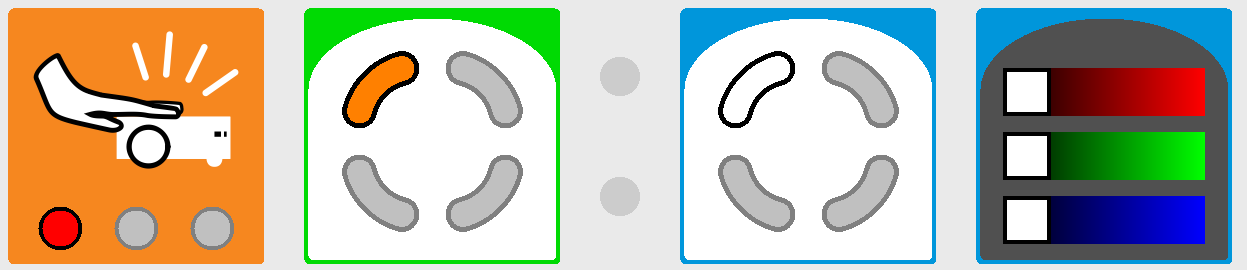
\includegraphics[width = 0.35\textwidth]{tap-on-off2}}
    \caption{Le programme complet avec deux types de paire événement-action}
    \label{fig.state-changing}
\end{figure}

Vous remarquerez le symbole \blk{states_icon} présent à côté de chaque événement. Ce symbole représente le mode dans lequel Thymio doit se trouver pour que l'action associée se déclenche. Chacune des quatre cases peut-être grise, blanche ou orange. Pour simplifier la suite du texte, nous allons numéroter les cases comme suit: \blk{states_icon_numbered}. Nous appelerons \textit{état}, la couleur d'une partie de ce cadran. Par exemple, Thymio pourra être en mode n$^\circ$1 si l'état de son cadran est [\textit{blanc, blanc, blanc, blanc}].

\begin{itemize}
	\item Une case \textbf{blanche} signifie \textit{état blanc}
	\item Une case \textbf{orange} signifie \textit{état orange}
	\item Une case \textbf{grise} signifie \textit{n'importe quel état}, \textit{blanc} ou \textit{orange}
\end{itemize}

Ainsi, sur \cref{fig.state-changing-a}, la première paire d'événement-action est déclenchée si Thymio est en \textit{mode éteint} avec le cadran équivalent [\textit{blanc, gris, gris, gris}]. En suivant ce concept, la deuxième paire d'événement-action action est déclenchée seulement si Thymio est en \textit{mode allumé} avec le cadran équivalent [\textit{orange, gris, gris, gris}]. 

\begin{bclogo}[couleur = blue!30, arrondi = 0.1, logo = \bcinfo, ombre = true]{Truc et astuce!}C'est à vous de choisir les modes de Thymio et d'y associer un état du cadran. Nous aurions très bien pu associé le \textit{mode allumé} à l'état  [\textit{orange, blanc, blanc, orange}] et le \textit{mode éteint} à l'état [\textit{blanc, orange, blanc, orange}]. Il aurait simplement fallu rester cohérent dans tout le programme. Mais avouez que les états du cadran que nous avons choisi sont plus simples. Essayez toujours de rester le plus simple possible!
\end{bclogo}

Pour que le programme soit complet, il ne faut pas simplement avoir des lumières qui s'allument ou s'éteignent en fonction du mode de Thymio mais il faut aussi changer le mode de Thymio! C'est là que \cref{fig.state-changing-b} entre en jeu. La première paire événement-action signifie: \textit{Si Thymio reçoit une tape et qu'il est en \textbf{mode éteint}, alors passer en \textbf{mode allumé}}. De même, la deuxième paire événement action signifie: \textit{Si Thymio reçoit une tape et qu'il est en \textbf{mode allumé}, alors passer en \textbf{mode éteint}}.

Nous avons donc deux actions qui sont lancées lorsqu'un événement "tape" est détecté. Un changement d'état d'un cadran (donc un changement de mode) et un changement de lumière.

\sect{Combien de modes pour Thymio?}

Nous avons vu que le mode de Thymio est donné par l'état d'un cadran divisé en quatre parties. Chaque partie peut-être en état blanc, orange ou gris. Un état gris signifiant n'importe quel état, si un mode est associé à \blksm{states}, alors, si Thymio se trouve dans le mode \blk{states1} ou \blk{states2}, l'action associée à cette paire sera déclenchée. Une case grise n'est donc pas un état à proprement parlé.

Il y a \textbf{quatre cases} qui peuvent être dans \textbf{deux états} différents. Les mathématiques nous disent donc qu'il peut y avoir $4^2 = 16$ modes! Ils sont tous illustrés sur \cref{fig.every-states}.

\begin{figure}[h]
    \centering
    \subfigure[Tous les états possibles de Thymio]{\label{fig.every-states} \includegraphics[width = 0.35\textwidth]{all_states}} 
    \hspace{1cm}
    \subfigure[La lumière indique le mode de Thymio]{\label{fig.state-leds} 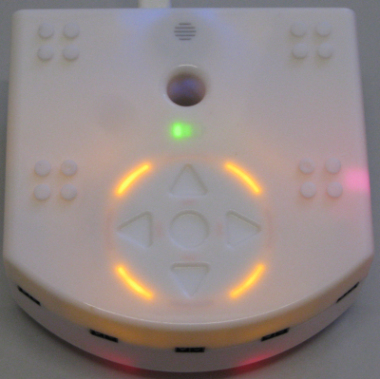
\includegraphics[width = 0.35\textwidth]{state-leds}}
    \caption{Les états de Thymio et leur représentation}
\end{figure}

Le mode de Thymio est physiquement illustré par des arcs de cercles lumineux. Le mode blanc éteint l'arc de cercle correspondant alors que le mode orange l'allume. \Cref{fig.state-leds} montre l'état complètement orange de Thymio.

\sect{Tête chercheuse}

\begin{bclogo}[couleur = pink!30, arrondi = 0.1, logo = \bccrayon, ombre = true]{Challenge!}Écrivez un programme en utilisant VPL qui fasse que Thymio tourne sur lui-même, dans le sens inverse des aiguilles d'une montre, à la recherche d'un objet. Lorsqu'il le repère avec son capteur tout à droite, Thymio doit tourner dans l'autre sens et s'aligner sur l'objet.
\end{bclogo}

{\raggedleft \hfill Programme \bu{tete-chercheuse.aesl}}

Comme il est aisé de représenter ce challenge avec un diagramme d'état, nous le donnons sur \cref{fig.State_diagram_mouse}.

\begin{figure}[h]
\begin{center}
\gr{State_diagram_mouse}{0.4}
\caption{Diagramme d'état}\label{fig.State_diagram_mouse}
\end{center}
\end{figure}

Pour réaliser ce programme, nous avons besoin de trois modes. 

\begin{itemize}
	\item Le \textbf{premier mode} est l'\textbf{arrêt}. Thymio est arrêté, il attend qu'on appuie sur son bouton central pour lancer la recherche. L'état du cadran associé à ce mode est 
\includegraphics[scale=0.3]{Mode1}
	\item Le \textbf{deuxième mode} est la \textbf{recherche}. Thymio cherche l'objet en tournant sur lui-même. Il ne sortira de ce mode que lorsqu'il verra l'objet sur son capteur tout à droite. L'état du cadran associé à ce mode est 
\includegraphics[scale=0.3]{Mode2}
	\item Le \textbf{troisième mode} est l'\textbf{alignement}. Thymio tourne dans l'autre sens pour s'aligner avec l'objet. Il ne sortira de ce mode que lorsqu'il verra l'objet en face de lui. L'état du cadran associé à ce mode est 
\includegraphics[scale=0.3]{Mode3}
\end{itemize}

En regardant les flèches et les indications de \cref{fig.State_diagram_mouse}, nous pouvons voir que:

\begin{itemize}
	\item Pour passer du mode 1 au mode 2, nous devons appuyer sur le bouton central de Thymio
	\item Pour passer du mode 2 au mode 3, Thymio doit trouver l'objet avec son capteur tout à droite
	\item Pour passer du mode 3 au mode 1, Thymio doit trouver l'objet avec son capteur central, il doit donc être aligné avec l'objet.
\end{itemize}

En suivant toutes ces indications, nous pouvons construire le programme illustré sur \cref{fig.prog_tete_chercheuse}.

\begin{figure}[h]
    \centering
    \subfigure[]{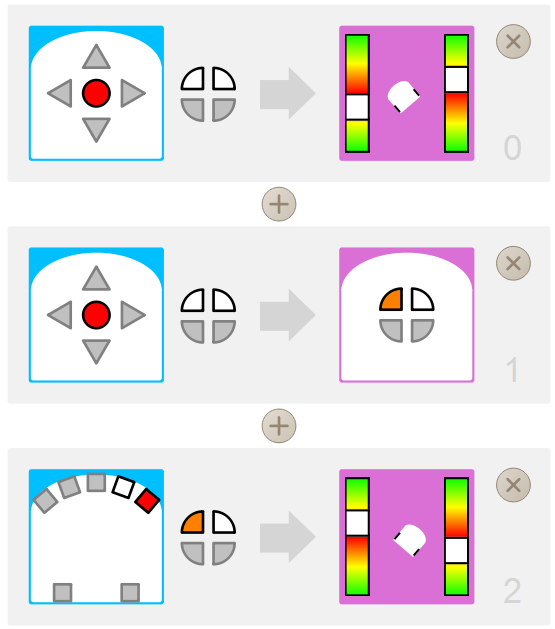
\includegraphics[width = 0.35\textwidth]{homing_thymio}} 
    \hspace{1cm}
    \subfigure[]{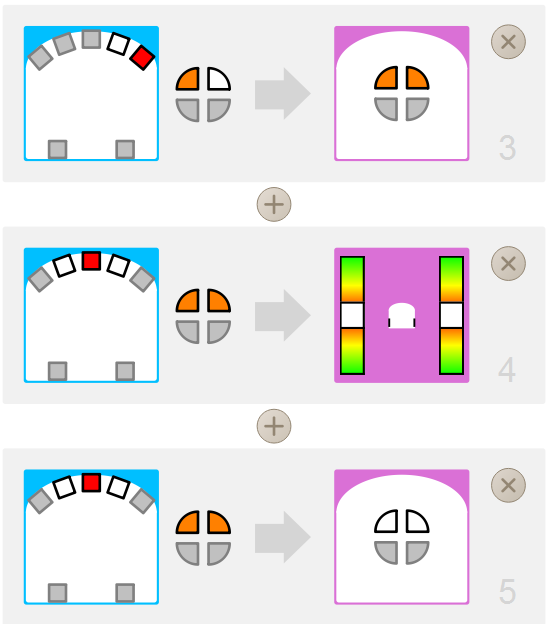
\includegraphics[width = 0.35\textwidth]{homing_thymio2}}
    \caption{Thymio tête chercheuse}
    \label{fig.prog_tete_chercheuse}
\end{figure}

\begin{bclogo}[couleur = pink!30, arrondi = 0.1, logo = \bccrayon, ombre = true]{Challenge!}Écrivez un programme en utilisant VPL qui fasse que Thymio devienne bleu lorsqu'il suit une ligne et qu'en cas de perte de la ligne, il devienne rouge et parte à sa recherche et ceci jusqu'à ce qu'il la retrouve.
\end{bclogo}
\chap{Et après?}

Ce tutoriel vous a présenté Thymio, Aseba et le VPL. Cet environnement de programmation par image est très pratique et simple d'emploi mais il a tout de même des limitations. Il n'est pas conçu pour programmer des comportements complexes. Pour cela, il vous faudra vous familiariser avec l'environnement d'Aseba Studio, comme illustré sur \cref{fig.Aseba_general}.

\begin{figure}[hbt]
\begin{center}
\gr{studio}{1}
\caption{L'environnement d'Aseba Studio}\label{fig.Aseba_general}
\end{center}
\end{figure}

La programmation en utilisant Aseba Studio est aussi basée sur les événements. On retrouve toutes les fonctionnalités que vous avez découvertes en utilisant le VPL. La vraie différence vient de la liberté quasi totale que vous aurez en programmant sur Aseba Studio.

Vous pourrez ajuster tous les tests conditionnels, par exemple sur le taux de lumière réfléchie sur un capteur. Les restrictions, comme "le capteur ne voit pas de lumière" ou "le capteur voit de la lumière", sautent. Vous pourrez tout régler très précisément.

Vous obtiendrez la liberté de travailler avec des variables, d'avoir de la mémoire, d'utiliser toute une batterie d'expressions, de tests\ldots

De plus, vous pourrez contrôler toutes les lumières, pas seulement le dessus et le dessous de Thymio. Vous aurez plus de flexibilité pour le contrôle du synthétiseur de son. Vous aurez accès à un capteur de température. Vous pourrez voir plus précisément les valeurs des accéléromètres sur les trois dimensions et plus seulement détecter un choc. Finalement, vous pourrez utiliser une télécommande pour contrôler Thymio!

Vous pouvez vous rendre sur le site web d'Aseba pour avoir plus d'informations et pour vous lancer dans la programmation \textit{écrite} et plus seulement \textit{visuelle}: \url{https://aseba.wikidot.com/fr:thymio}

Il est possible d'importer dans Aseba Studio tous les programmes qui proviennent du VPL en les ouvrant simplement dans Asbea Studio.

Il ne vous reste plus qu'à tester Thymio sous toutes les coutures! Si vous manquez d'inspiration, allez faire un tour sur la page des exemples du site web d'Aseba, vous y trouverez de nombreux nouveaux challenges!

\begin{figure}[h]
\begin{center}
\gr{Thymio_bye}{1}
\end{center}
\end{figure}
\end{document}
